\chapter{Stochasticity of the evolution}
In the previous chapters, we derived an approximated expression for the exit times using the high-dimensional
ordinary differential equations of the process.
The results obtained were only partially satisfactory, as they only partially captured the exit-time trend,
allowing us to make assertions only about the orders of magnitude of the gain obtained by overparameterizing the neural network.

In this chapter we will introduce corrections to the differential equations we have previously used,
transforming them into stochastic differential equations, with the aim of having an exact expression of exit-time.
We will focus only on the phase retrivial, given the simplicity of the equations it involves. 

\section{Stochastic differential equations}
There are two main problems affecting the results on the exit times of previous chapter.
The first one is that the differential equation are valid in the limit~\(d\to+\infty\),
but then we use big, but still finite, \(d\) for comparsion. 
The second problem is that Theorem~\ref{thm:process_to_ode_goldt} explicitly says that the solution of the differential equation approximates the trajectories with an accuracy that scales as \(\frac{1}{\sqrt{d}}\),
which is of the same order as the variation in the order parameters we are trying to measure.
Although we collect some statistics by simulating different trajectories,
the differential equations do not seem to be sufficient to have an accurate estimate of the exit time.

The ordinary differential equations were derived as the limit of a discrete stochastic process.
All random components were cancelled by the limit procedure, leaving simply the expectation value of the random variable.
Rewriting the Equations~\eqref{eq:genericODE}, in the case \(k=p=1\) we have 
\[\begin{split}
  \dod{\left[\M{\left(t\right)}\right]_{11}}{t} &=\E_{\vec{\lf},\vec{\lf^* \sim \gauss{(0,\vec{\Omega}{(t)})}}}{\left[\mathcal{M}\right]} \\
  \dod{\left[\Q{\left(t\right)}\right]_{11}}{t} &=\E_{\vec{\lf},\vec{\lf^* \sim \gauss{(0,\vec{\Omega}{(t)})}}}{\left[\mathcal{Q}\right]},
\end{split}\]
where we have introduced the two random variables
\[\begin{split}
  \mathcal{M} \coloneqq &  \frac{\gamma}{p} \dsp_1 \lf_1^* \\
  \mathcal{Q} \coloneqq &  \frac{\gamma}{p}\left(\dsp_1 \lf_1 + \dsp_1 \lf_1\right) + \frac{\gamma^2}{p^2} \dsp_1^2
\end{split}\]
What we want to do is to include correction terms that incorporate the next order in \(d\).
Obviously, the correction cannot be deterministic since the limit is computed on a random variable;
moreover, it will have to have zero expectation value, otherwise, it would go to change order 0.
The simplest model we can imagine is given by introducing white noise that has as its intensity the standard deviation of the variables on which the expectation values are computed.
In other words, in the passage to the limit, instead of turning the random variables into expectation values,
we instead replace them with Gaussians that best approximate the random variables.
Let's put these considerations into formulas. We can start by defining the covariance matrix of \(\mathcal{M}\)
and \(\mathcal{Q}\)
\[
  \vec{\Sigma} \coloneqq 
  \begin{pmatrix}
    \Var{\left[\mathcal{M}\right]} & \Cov{\left[\mathcal{M},\mathcal{Q}\right]} \\
    \Cov{\left[\mathcal{M},\mathcal{Q}\right]} & \Var{\left[\mathcal{Q}\right]}
  \end{pmatrix},
\]
from which we can define the standard deviation vectors
\[
  \begin{pmatrix}
    \vec{\sigma}_m \\
    \vec{\sigma}_q
  \end{pmatrix}
  \coloneqq
  \sqrt{\vec{\Sigma}}.
\]
We introduce the noise as a differential vector of Wiener processes, one per equation
\[
  \dif \vec{W} \coloneqq 
  \begin{pmatrix}
    \dif W_m \\
    \dif W_q
  \end{pmatrix}
\]
where \(W_m\) and \(W_q\) are 2 indipendent Wiener processes.
What was previously a system of ordinary differential equations now becomes a system of stochastic differential equations.
Referring to Equations~\eqref{eq:genericODE} for notation, and eliminating subscripts since we are focusing on phase retrivial
\begin{subequations}\begin{align}
  \dif m =& \Psi{(m,q)}\dif t + \frac{\vec{\sigma}_m{(m,q)}\cdot\dif \vec{W}}{d} \\
  \dif q =& \Phi{(m,q)}\dif t + \frac{\vec{\sigma}_q{(m,q)}\cdot\dif \vec{W}}{d} 
\end{align}\end{subequations}
Obviously in the limit \(d\to+\infty\) we fall back to ordinary differential equations,
since the stochastic term cancels out.
These equations describe the evolution of the unconstrainted phase retrivial,
which will be the first case we are going to analyze in the next section.

\subsection{Initial conditions}
Before we go to simulate the stochastic process, we must choose what initial conditions to use.
Since our goal is to find a description of the learning process that is able to detect effects that escaped the differential equations,
we will look at the situation where they strayed furthest from the simulation. 
We therefore choose to initialize the phase retrivial with the \emph{symmetric intial conditions with \(\varepsilon = 0\)} (see the \ref{subsec:symmetric_init} section).
In our context we can also assume \(q_0 = 1\): this basically means choosing the vectors \(\w\) and \(\w^*\) as orthogonal
\[
  q(0) = 1, \quad m(0) = 0 \quad\text{and}\quad\rho=1.
\]

As already shown, the description with differential equations is not able to break the initial symmetry and the vectors remain orthogonal throughout the process,
changing only the norm of \(\w\).
In contrast, we expect the stochasticity introduced by the corrective term to lead to symmetry breaking and a consequent correct description of the learning process.

Finally we choose to study the case with \(\Delta=0\). 
This choice follows from the fact that in the past chapters we have shown that the value of noise only marginally affects the first part of the process,
i.e., the part we want to study. We therefore choose to exclude it in order to have a less complex,
but no less descriptive, description of the process.


\section{Unconstrainted Phase retrivial}
We can now turn to testing the model we introduced in the previous section.
The value of \(\Phi\) and \(\Psi\) is known from Equations~\eqref{eq:phase_retrivial},
while the matrix \(\vec{\Sigma}\) is calculated in Appendix~\ref{app:std_sde}.

\begin{figure}
  \centering
  \begin{subfigure}{0.75\textwidth}
    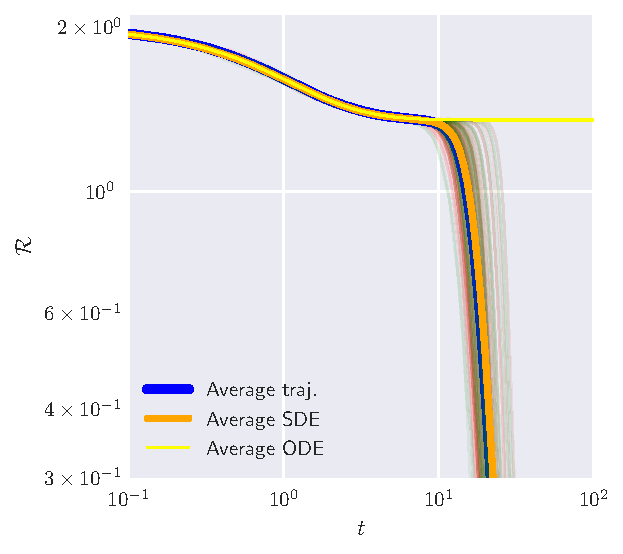
\includegraphics[width=1.\textwidth]{figures/sde/unconstrainted-sde-example.pdf}
    \caption{general trend}
  \end{subfigure}
  \begin{subfigure}{0.75\textwidth}
    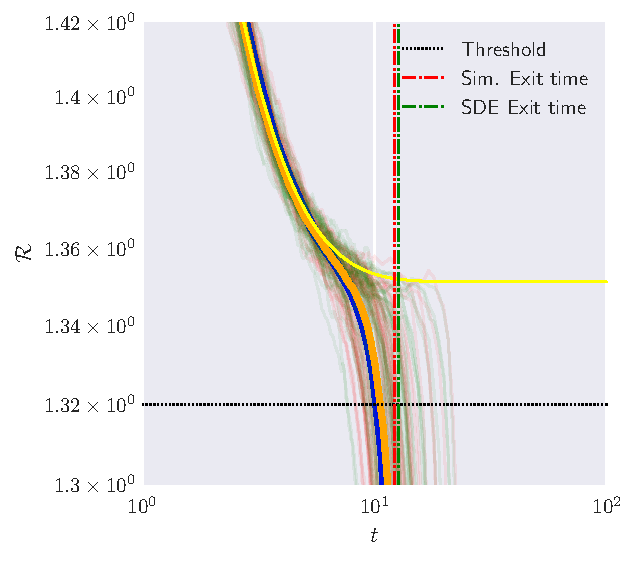
\includegraphics[width=1.\textwidth]{figures/sde/unconstrainted-sde-example-zoom.pdf}
    \caption{zoom on separation zone}
  \end{subfigure}

  \caption{
    comparison between simulation and theory with \(\gamma=\num{0.1}, \Delta=0\).\\
    The shaded red lines represent the different simulated trajectories,
    while the shaded green lines are different realizations of the solution of the stochastic process.
  }
  \label{fig:unconstrainted-sde}
\end{figure}
Figure~\ref{fig:unconstrainted-sde} shows the result of a simulation.
The first thing to observe is that, as we expected, the solution of the differential equations is not able to break symmetry.
Conversely, the description through the stochastic process is not affected by this problem,
being able to emulate the results obtained by training the complete network.

In the figure, the individual trajectories used to evaluate both the simulation and the process obtained from the SDEs are also shown:
we can see how the distributions seem to overlap, a symptom of the fact that the stochastic process has the same distribution as the complete network.
As evidence for this claim, we calculated two different statistics to compare:
the average trajectory and the time to exit a threshold.
Both coincide within the experimental error, which, however, cannot be eliminated having used a finite number of samples (56 for each).

The result is in agreement with what was recently reported in a paper by G. Ben Arous et al.\cite{arous2022high}.
% todo: spiega il paper di Ben Arous

\section{Spherical Phase retrivial}
\subsection{Naive derivation}
\subsection{Itô}



